

\documentclass[12pt]{extarticle} % set to 12 when done

\usepackage{outlines}
\usepackage{graphicx} % Add pictures to your document
\usepackage{listings} % Source code formatting and highlighting
\usepackage{amsmath}
\usepackage{amsthm}
\usepackage{extsizes}
\usepackage{amsfonts} 

\usepackage[margin=0.5in]{geometry}


\graphicspath{ {./pics/} }


\begin{document}
\newcommand\abs[1]{\left|#1\right|} % absolute
\newcommand\magnitude[1]{\left\Vert #1 \right\Vert}
\newcommand\vectoo[1]{\begin{bmatrix} #1 \end{bmatrix}}
\newcommand{\seq}[2][0]{\left\{ #2 \right\}_{n=#1}}
% ^ newcommand, use like \seq[startingg_n]{sequence}
\newtheorem{theorem}{Theorem}
\newtheorem*{theorem*}{Theorem}
\newtheorem*{definition}{Definition}

\section{Algemene begrippen}

\subsection{Symbolen}


    W = arbeid \\
Q = warmte \\
c = soortelijke warmte \\
$\eta$ = rendement \\
U = inwendige energie \\
H = entalpie \\ 
S = entropie


\subsection{Soortelijke warmte}

De hoeveelheid warmte die aan een stof toegevoerd moet worden om van T1 naar T2 te gaan,
indien de c constant is -wat het meestal niet is- , 
kan beschreven worden als

$$
    Q_{12} = m c (T_2 - T_1)  
$$, waar c de soortelijke warmte van een stof is. De soortelijke warmte wordt uitgedrukt in ${kJ \over kg \cdot K}$
, en is afhankelijk van de tempperatuur en druk(verwaarloosbaar bij vloeistoffen en vaste stoffen).
Soms krijg je een functie voor c, zoals $c(T) = a + bT$, soms gebruik je de gemiddelde waarde, en soms moet je het gewoon interpoleren vanuit een tabel. 
Indien je het interpoleerd van een tabel krijg je dan een c1 en c2, die je dan zo gebruikt om warmte te berekenen:
$$
Q_{12} = m (c_2  T_2 - c_1 T_1)
$$

Indien je een functie krijgt, dan moet je gewoon integreren, zoals hier:
$$
\int dQ = \int m c(T) dT
$$

De bovenstaande manieren zijn beide gewoon afgeleid van de volgende functie:

\begin{equation}\label{eq:warmte DE}
    dQ = m \cdot c(T) dT \\
    \end{equation}
Meestal kan er gewoon geworken worden met de gemiddelde soortelijke warmte ( $\bar{c}$ ), wat je zo berekent:

\begin{equation}\label{avg. soortelijke warmte}
    c_{12} = {c_2T_2 - c_1T_1 \over T_2 - T_1}
\end{equation}

\subsection{ Verbrandingswarmte en stookwarmte}

\textbf{Verbrandingswarmte} is de hoeveelheid energie die vrijkomt als iets verbrand wordt. Hierbij is de energie die vrijkomt bij het condenseren van water inbegrepen.

\textbf{Stookwarmte} is de verbrandingswarmte minus de warmte die vrijgegeven wordt als het water condenseert. Dit is meestal practischer, want de condensatiewarmte
gaat meestal verloren.

De bovenstaande worden meestal in ${kJ \over kg}$ of $kJ \over m^3$ weergeven.


\subsection{Rendement}
In vele instalaites vinden er energie omzettingen plaatst, en men tracht zo veel mogelijke nuttige energie te verkrijgen 
uit de ingevoerde energie/arbeid. De ratio tussen deze wordt rendement genoemt.

\begin{equation*}
    Rendement(\eta) = {E_{out} \over E_{in}} = {W\over Q}
\end{equation*}
waar W de warmte is.

\subsection{Gassen en mengsels}
Dit is de gaswet, en is beperkt tot \textbf{idiale} gassen. 

\begin{equation}
    {p_1 V_1 \over T_1} = {p_2 V_2 \over T_2}
\end{equation}

Verder kan je een toestandsvariabel berekenen als het ontbreekt dmv de toestandsvergelijking:
\begin{equation}\label{toestandsvergelijking}
    p V = m R T 
\end{equation}
waar m de hoeveelheid mol x de molmassa is. 
\textbf{Het is belangrijk om te onthouden dat de bovenstaande alleen voor idiale gassen gelden.} Bij hoge drukken begint de echte
gedrag steeds meer af te wijken van wat deze vergelijkingen beschrijven.


\subsection*{Schoolnotes}
$E_{molecuul} = E_{kin} + E_{pot}$
Kinterische energie is gekkopeld aan de temperatuur. Voor elke vrijheidsgraad heb je dit aan energie:
$$
0.5 {m\over v^2} = 1.5 K \cdot T
$$
waar k de boltzman constante is.

\begin{equation}\label{1e hoofdwet}
    dE_{inwendig} = dQ + dW
\end{equation}

\subsubsection{Arbeid}
Een gas- en vloeistofdruk is altijd loodrecht op de wanden. 
mechanische arbeid:  $W - F \cdot S \cdot cos \alpha$ (voornamelijk voor zuigers nodig)

De Q die toegevoegd wordt bij faseverandering gaat naar het breken van bindingen.

in differentiaalvorm kan gezecht worden:

$$
dW = d(p\cdot v) = \int V dp + p dv
$$
Maar voor een quasistatische proces (een proc. die heel langzaam verloopt, we nemen aan dat alle processen heel langzaam lopen)
 kan gezegt worden dat dp = 0, dus :
 $dW = \int p d v$
 En dit is de arbeid verricht door een expanderende gas.

 De arbeid die verricht wordt(of nodig is) door een proces kan als volgt beschreven worden 

 \subsubsection{Isobaar}
 Een isobaar proces is een proces waar de druk constant blijft. 

 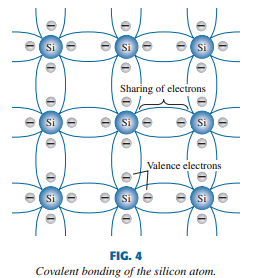
\includegraphics{2.png}
 De algemene formule om de W te berekenen voor alle processen is als volgt:

 $$
 W = \int_Va^Vb p dv = p(V_b-V_a)
 $$
 Note dat v een functie zou kunnen zijn
 Een isochoor process is waar de volume constant blijft.
 Er wordt geen arbeid uitgevoerd.

 Een isotherm is waar de temp constant blijft. 
$$
W = \int p dv
$$

Een proces is wanneer een stof van een toestand naar een andere toestand gaat. Ze worden polytropen genoemd, 
en de volgende zijn gewoon bijzondere polytropen:
\begin{itemize}
    \item isobaar : n = 0, p = constant dus $p v^0 = C$
    \item isochoor: n  dus $p v^\infty = C$
    \item isotherm: n = 1, p = constant, dus $p v^1 = C$
    \item adiabaat : $p v^n = C, n = {c_p \over c_v}$
\end{itemize}
De algemene formule voor een polytroop is $konstant = p v^n$, en deze moet dan hetzelfde zijn voor en na de process.

dus $(p v^n)_{\text{in a}} = (p v^n)_{\text{in b}}$



\end{document}









